\chapter{実装}
{
\label{chap:implement}
本章では\ref{chap:parallel}章の並列化に対する検討を元にして、FPGAに実装するアクセラレータについて解説する。
\section{スレッド並列化の実装}
\label{sec:thread_impl}
図\ref{fig:para_inception}で示した4つの計算スレッドについて、各スレッドにそれぞれ1枚のFPGAで演算を行うようにする。

\section{スレッド内モジュールの実装}
\label{sec:module_impl}
FiCのマルチFPGAシステムでは、流れてきたデータをそれぞれのFPGAボードでの処理を終えて、次のFPGAに出力を渡す、というフローが想定される。
そのため各ボードでは特定の演算処理のみを実行すればよいので\cite{optimized}のように複数のサイズの畳み込みを行うことは考えずに、
それぞれの層に適した入出力サイズのモジュールを実装することが可能である。また特定の層の重みフィルタのみをBRAMに保存して読み出し演算を行う。
各スレッドのモジュールはまず、ブロードキャストされる同一サイズの入力値を受け取る。BRAMの重みフィルタとの畳み込み演算を行う。
% 図\ref{fig:thread_module}にモジュールの模式図を示す。

% \begin{figure}[h]
%     \centering
%     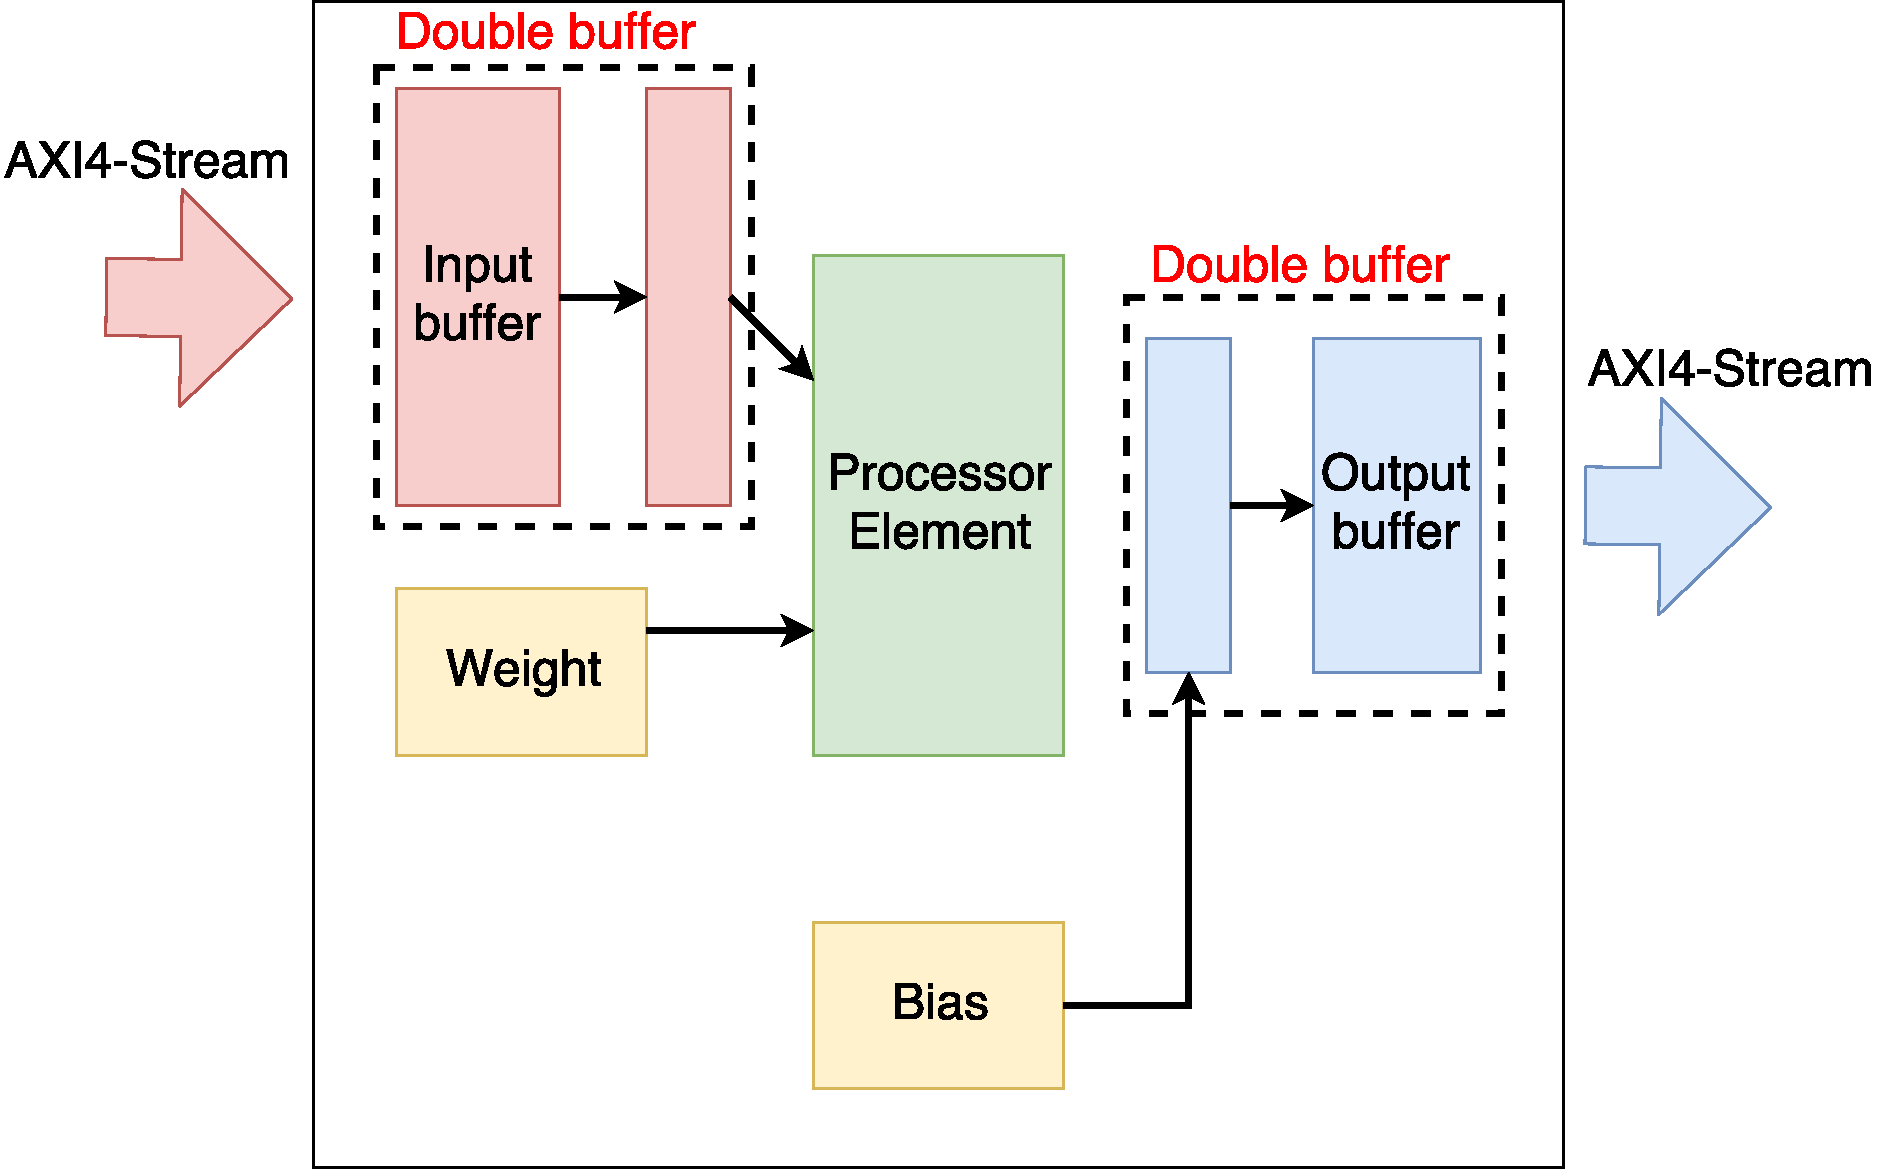
\includegraphics[width=12cm]{./chap6/fig/thread_module.pdf}
%     \caption{モジュールの模式図}
%     \label{fig:para_inception}
% \end{figure}

入出力にダブルバッファを設けることで、ストリーム処理を可能にし、演算に必要なデータが揃ったら演算を行うと同時に次のデータを書き込むことができる。
畳み込み演算はPEで行う。図\ref{fig:para_inception}で示した4つの計算スレッドのうちthread2、thread3,thread4については畳み込みやpooling処理
が連続して行われているので図\ref{fig:thread_module}が2つ接続するようなモジュールとなる。

\section{畳み込み演算器の実装}
\label{sec:conv_impl}
\ref{sec:module_impl}節で述べたモジュールの模式図内のPE部の設計は\cite{optimized}を参考にした。
% ここでは\ref{code:conv}に示す、畳み込み演算の疑似コードをループタイリングによって分割することで並列化することを考える。
% \ref{code:conv_tile}がループタイリングを行った疑似コードである。$T_m$、$T_n$がそれぞれ入力値、出力値のタイルのサイズとなっている。
この疑似コードに倣って演算モジュールを作ると図\ref{fig:conv_pe}のような演算器を設計できる。

\begin{figure}[h]
    \centering
    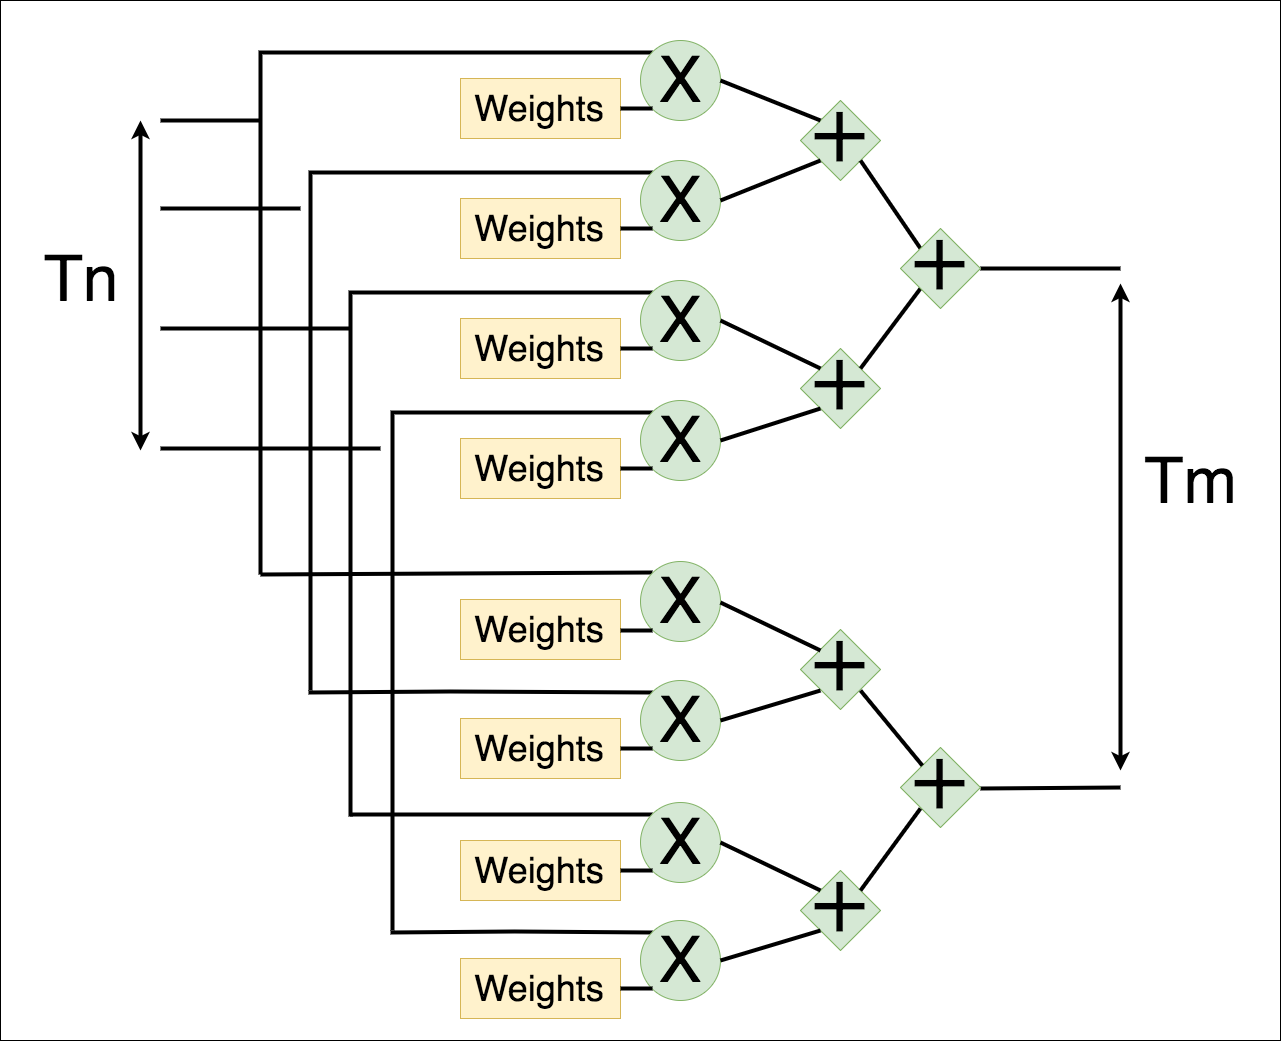
\includegraphics[width=12cm]{./chap6/fig/ucla_pe.png}
    \caption{畳み込み演算器の模式図}
    \label{fig:para_inception}
\end{figure}
% 畳み込み演算器のタイリングしたモジュールの説明を入れる。
}

